\documentclass[../midgard.tex]{subfiles}
\graphicspath{{\subfix{../images/}}}
\begin{document}

\section{Time model}
\label{h:time-model}

Midgard partitions time in two different ways:
\begin{description}
    \item[Operator shifts.] Predefined, non-overlapping time intervals assigned to operators by the Midgard scheduler.
      Each operator has the exclusive privilege to commit blocks to the state queue and resolve nodes in the settlement queue during their assigned shifts.
      If an operator fails to commit blocks regularly in their shift, the next operator can take over.
    \item[Event intervals.] Emergent, non-overlapping time intervals claimed by operators' committed blocks.
      Each operator block is expected to include all user events with inclusion times within its event interval and to exclude all other user events.
      For L1 user events (deposits, transaction orders, withdrawal orders), this is enforced by Midgard's ledger rules.
\end{description}

Operator shifts are evenly sized according to the \code{shift\_duration} Midgard protocol parameter.
The scheduler assigns operators to shifts by iterating over the list of active operators in key-descending order, allowing new operators into the list at the end of each cycle.
The state queue enforces this schedule by requiring the time-validity upper bound of every block commitment transaction to fall within its operator's shift.

During a shift, an operator is expected to commit blocks to the state queue at a regular cadence.
However, Cardano's L1 consensus protocol introduces randomness into this process, so the operator does not know in advance at which precise time and block their block commitment transaction will be confirmed.
In practice, each block commitment transaction must set a fairly long time-validity interval (e.g., 5 minutes) to have a reasonable probability of confirmation on L1.
On the other hand, the operator will often see the transaction confirmed much earlier than the end of this time-validity interval, so they have little reason to wait after confirmation to commit the next block.\footnote{In fact, an operator may commit blocks without waiting for L1 confirmation.
As long as the blocks are valid, no one can interfere with the operator's chain of block commitment transactions.
Moreover, if operators coordinate their activity offchain, this rapid cadence can be mostly maintained across shift boundaries.}

In this way, consecutive blocks will overlap significantly in their time-validity intervals, but each block's time-validity upper bound will likely be shifted forward by a random amount relative to its predecessor so that it has a similar probability of confirmation.
Furthermore, the state queue enforces that each block's time-validity lower bound must be within its predecessor's time-validity interval.
Therefore, the sequence of block time-validity intervals induces a partitioning of time, whereby each block's event interval is the portion of its time-validity interval that occurs after its predecessor's time-validity interval.

\begin{figure}[htb]
\centering
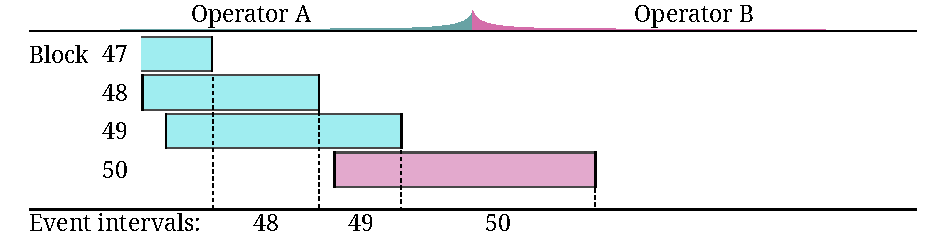
\includegraphics[scale=1]{\subfix{../images/time-model.pdf}}
\caption{Midgard time model.
Each rectangle shows a block's time-validity interval and its relationship to the operator windows (top axis) and event intervals (bottom axis).}
\label{fig:time-model}
\end{figure}

\end{document}
